\begingroup
\emergencystretch=3em
\section{Результаты}
\subsection{Условия проверки}
Замеры производительности выполнены 12.11.2026 на компьютере студента
с процессором Intel Core i7-13650HX в WSL2.
Система: Linux 6.6.87.2-microsoft-standard-WSL2, x86-64, glibc 2.39.
Среде доступны 20 логических CPU. Использована текущая версия лабораторной
с интерфейсом \texttt{mt}, собранная CMake в режиме Release.
Версия компилятора в журнале окружения не зафиксирована.
Исходные результаты: \texttt{inc/measurements/raw.csv};
итоговая таблица: \texttt{inc/measurements/summary.csv};
сведения о системе: \texttt{inc/measurements/environment.txt}.

Следующие проверки небольшой матрицы и количества потоков относятся
к ранее подготовленной контрольной Linux-сборке. Они приведены отдельно
и не являются журналами новых замеров на компьютере студента.

\subsection{Проверка на небольшой матрице}
Для исходной матрицы
\[
A=\begin{pmatrix}1&2&3\\4&5&6\\7&8&9\end{pmatrix}
\]
при \(K=1\), \(W=3\) получены
\[
E=\begin{pmatrix}1&1&2\\1&1&2\\4&4&5\end{pmatrix},\qquad
D=\begin{pmatrix}5&6&6\\8&9&9\\8&9&9\end{pmatrix}.
\]
Они совпали с независимо рассчитанными ожидаемыми значениями
при одном и трёх участниках. При \(K=2\) все элементы результата
эрозии равны 1, а наращивания --- 9.

Дополнительно проверены \(K=0\), окно \(1\times1\) при пяти проходах,
запрос 20 потоков для трёх строк, а также отклонение параметров
\texttt{-t 0}, \texttt{-k -1}, \texttt{-w 2}.
Все девять перечисленных проверок завершились согласно ожиданиям.
Журнал проверок:
\lstinputlisting[language={},basicstyle=\footnotesize\ttfamily,numbers=none]{inc/checks.txt}

Фактический журнал запуска с тремя участниками:
\lstinputlisting[language={},basicstyle=\scriptsize\ttfamily,numbers=none,breaklines=true]{inc/small.log}
PID у участников одинаков, а TID различаются. Диапазоны строк
не пересекаются. Порядок диагностических строк зависит от планировщика.
Время короткого запуска с \texttt{-v} не используется для оценки ускорения.

\subsection{Подтверждение количества потоков средствами ОС}
Для достаточно длительного запуска матрицы \(1024\times1024\),
\(K=100\), \(W=5\), \(P=4\) выполнена команда
\begin{lstlisting}[language=bash,numbers=none]
ps -L -p "$pid" -o pid,tid,nlwp,comm
grep '^Threads:' /proc/"$pid"/status
\end{lstlisting}
Фактический вывод \texttt{ps}:
\lstinputlisting[language={},basicstyle=\footnotesize\ttfamily,numbers=none]{inc/ps_threads.txt}
Фрагмент \texttt{/proc/PID/status}:
\lstinputlisting[language={},basicstyle=\footnotesize\ttfamily,numbers=none]{inc/proc_threads.txt}
Обе проверки фиксируют четыре системных потока: главный
и три дополнительных. PID и TID в этих журналах относятся только
к данному запуску, а не являются постоянными значениями программы.

\subsection{Методика измерения производительности}
Использованы матрицы \(256\times256\) и \(1024\times1024\),
\(K=10\), окно \(5\times5\) и \(P\in\{1,2,4,8\}\).
Для каждой конфигурации выполнен один прогревочный запуск и пять
измеряемых. В каждом повторе порядок значений \(P\) перемешивался
с фиксированным начальным состоянием генератора 12.
В итоговую таблицу занесена медиана пяти измерений.

Матрицы являются специально созданными тестовыми входами, а не
внешними экспериментальными данными: Python \texttt{random.Random(12+N)}
генерировал целые значения от \(-100000\) до \(100000\), делённые на 100.
Для всех чисел потоков проверено побайтовое совпадение двух выходных
файлов с однопоточным результатом по SHA-256.

Время берётся из \texttt{TIME\_SECONDS}. Оно включает создание
дополнительных потоков, вычисления, ожидания на барьерах, присоединение
потоков и освобождение их дескрипторов. Чтение исходного файла,
предварительное выделение и копирование матриц, а также запись результатов
за пределами этого интервала. Подробный вывод \texttt{-v} отключён.

Для фиксированных входных данных ускорение и эффективность определяются как
\[
S_p=\frac{T_1}{T_p},\qquad \eta_p=\frac{S_p}{p}.
\]
Здесь \(T_1\) и \(T_p\) --- медианы времени при одном и \(p\) участниках.
В таблице эффективность указана в процентах.

\begin{center}
\begin{tabular}{|r|r|r|r|r|}
\hline
Размер \(N\) & Потоки \(p\) & \(T_p\), с & \(S_p\) & \(\eta_p\), \% \\ \hline
256 & 1 & 0.018712 & 1.000 & 100.0 \\ \hline
256 & 2 & 0.011057 & 1.692 & 84.6 \\ \hline
256 & 4 & 0.011265 & 1.661 & 41.5 \\ \hline
256 & 8 & 0.013531 & 1.383 & 17.3 \\ \hline
1024 & 1 & 0.284596 & 1.000 & 100.0 \\ \hline
1024 & 2 & 0.147220 & 1.933 & 96.7 \\ \hline
1024 & 4 & 0.080648 & 3.529 & 88.2 \\ \hline
1024 & 8 & 0.072673 & 3.916 & 49.0 \\ \hline
\end{tabular}
\end{center}

\begin{figure}[htbp]
\centering
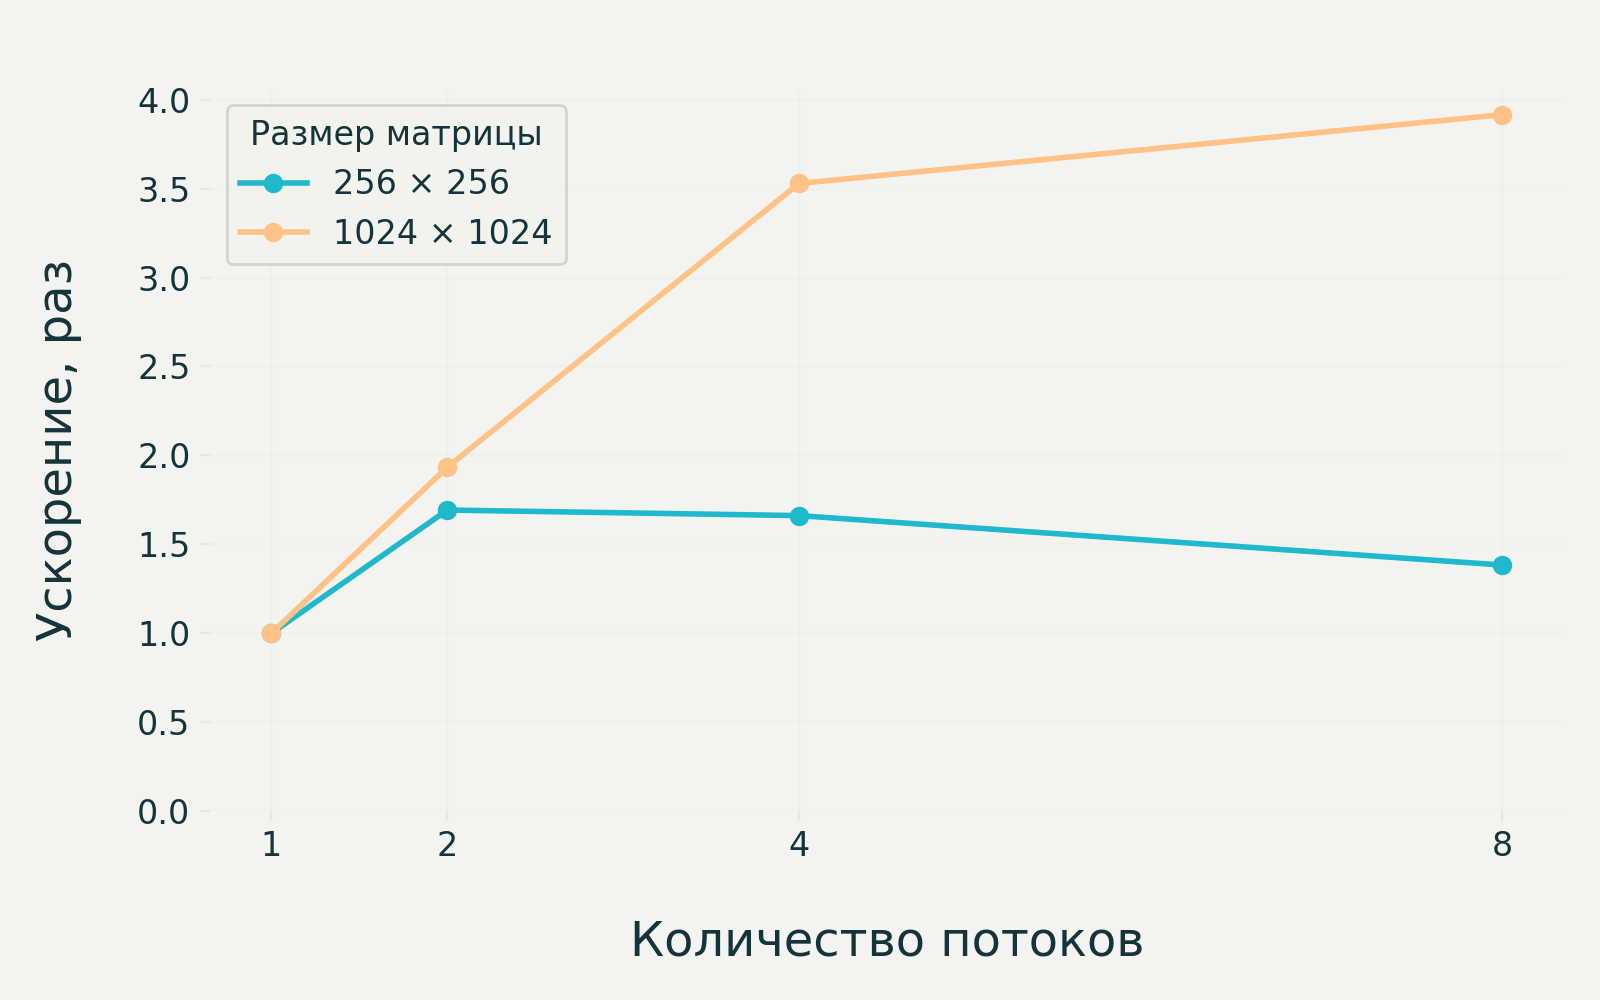
\includegraphics[width=0.95\linewidth]{img/speedup.png}
\caption{Ускорение: \(K=10\), \(W=5\).}
\end{figure}

\begin{figure}[htbp]
\centering
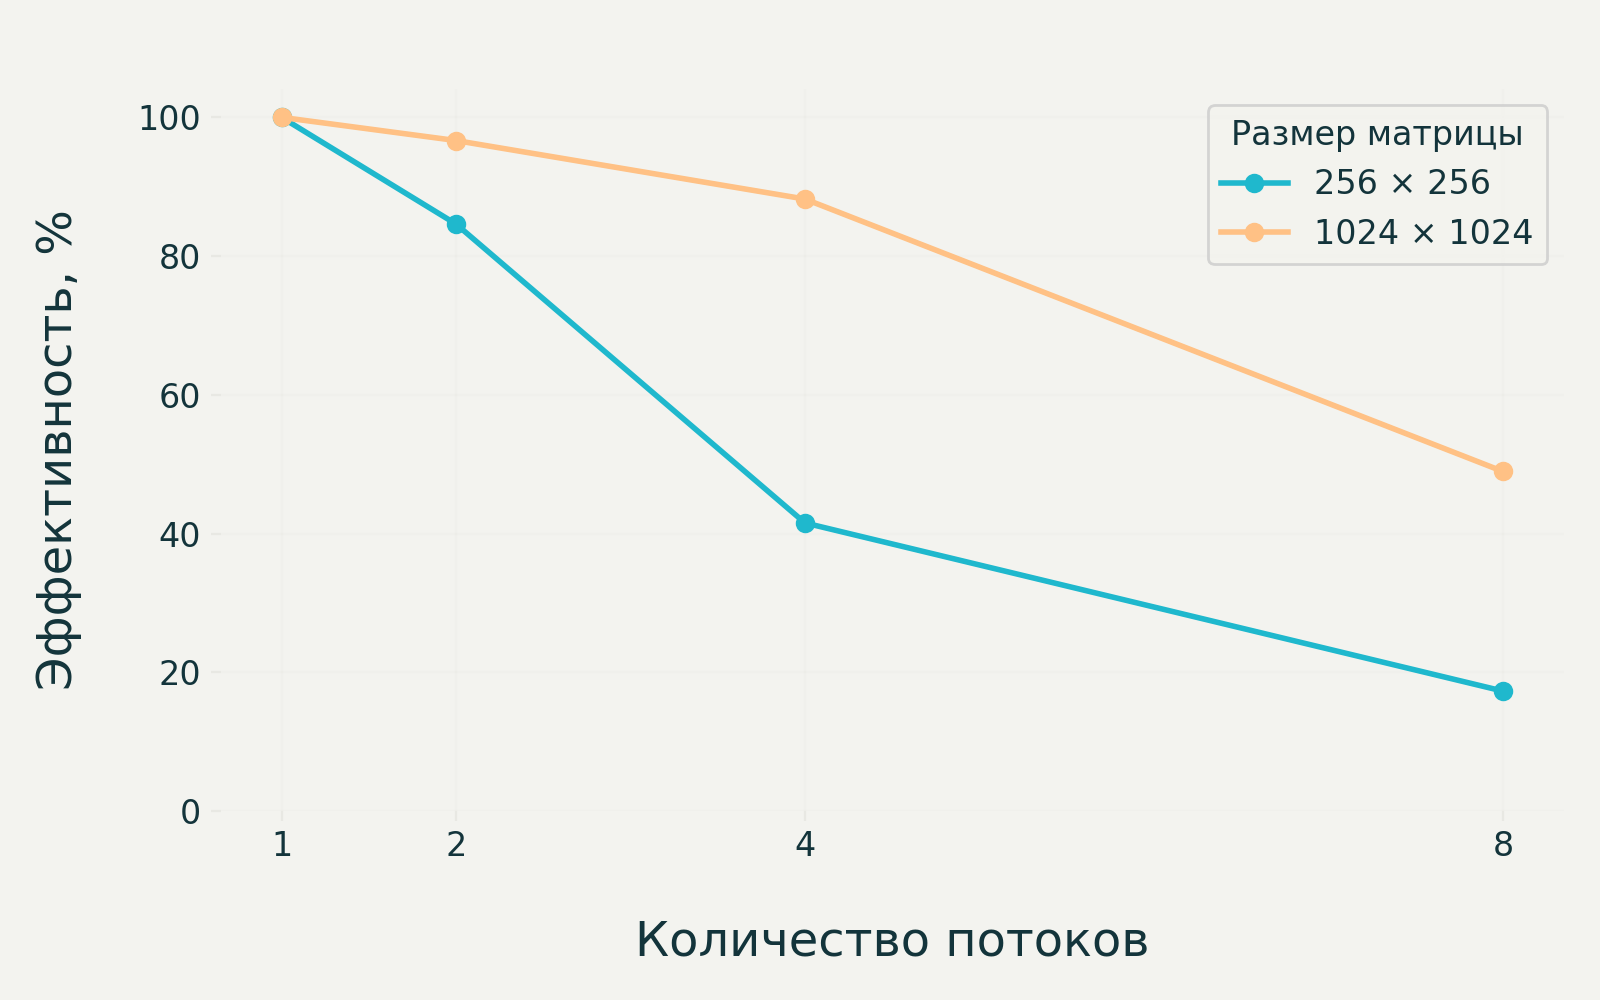
\includegraphics[width=0.95\linewidth]{img/efficiency.png}
\caption{Эффективность при изменении числа потоков.}
\end{figure}
\clearpage

\subsection{Объяснение результатов}
Для матрицы \(256\times256\) минимальная медиана времени получена
при двух потоках: 0.011057 с против 0.018712 с при одном.
Ускорение составляет 1.692, эффективность --- 84.6\%.
При четырёх потоках время равно 0.011265 с, при восьми --- 0.013531 с.
Для небольшой задачи увеличение числа потоков не обеспечило
дальнейшего уменьшения медианы времени.

Для матрицы \(1024\times1024\) медиана снизилась с 0.284596 с
при одном потоке до 0.147220 с при двух, 0.080648 с при четырёх
и 0.072673 с при восьми. Максимальное наблюдаемое ускорение
равно 3.916, эффективность восьми потоков --- 49.0\%.
Эффективность двух и четырёх потоков составляет 96.7\% и 88.2\%.

Результаты отдельных повторов различаются. Например, для матрицы
\(256\times256\) при двух потоках время находится в диапазоне
от 0.009704 до 0.029825 с. Поэтому в таблице и на графиках
использованы медианы пяти повторов, а не минимальные значения.
По этому эксперименту нельзя однозначно установить причины разброса;
влияние фоновой нагрузки, планировщика и виртуализации отдельно
не измерялось. Малое различие медиан двух и четырёх потоков
на небольшой матрице не доказывает устойчивого превосходства.

Восемь конфигураций дали 40 измеряемых запусков после прогрева.
Наличие 20 доступных логических CPU не означает линейного ускорения:
время включает создание потоков, вычисления, барьеры и ожидание завершения.
Полученные результаты относятся к указанной сборке и среде WSL2.
\clearpage
\endgroup
